
Here we perform a preliminary study on potential inversion schemes. We use various inversion schemes to recover an unknown bathymetry using a mock forward model and manufactured data. This preliminary work aided in the selection process of the three inverse methods chosen for this project.

\subsection{The Additive Gaussian Noise Model} \label{Gaussian_noise}
To accurately mimic the real problem, we create ``measurements'' that are corrupted by the Gaussian noise; this can be written as 
\begin{equation}
\mathbf{d} \sim \text{Gaussian}( \mathbf{A} \mathbf{h}_t),
\end{equation}
\vspace{0.3cm}
where\\
\begin{tabular}{l c l}
$\mathbf{d}$ &=& a vector of measurements,\\
$\mathbf{A}$ &=& a linear forward operator,\\
$\mathbf{h}_t$ &=& the true bathymetry (depth). 
\end{tabular}

\vspace{0.3cm}
Defining $\boldsymbol{\epsilon}$ as our Gaussian noise with a standard deviation $\nu$, the corrupted measurements can be represented as

$$
\mathbf{d} = \mathbf{A} \mathbf{h}_t + \boldsymbol{\epsilon}.
$$



\subsection{Ordinary Least-Squares Inversion}

%\subsubsection{Least-Squares Inversion}

To start,  we consider the following least-squares problem,
\begin{equation}\label{LS}
\mathbf{\hat{h}}= \underset{\mathbf{h} \in \mathbb{R}^n}{\arg \min} \ \ f(\mathbf{h}) = \|  \mathbf{A}\mathbf{h} -  \mathbf{d} \|_2^2,
\end{equation}
where we minimize the data misfit between the forward predictions and the measurements, in the least-squares sense. In order to test possible Matlab\textsuperscript{\textregistered} inbuilt solvers to solve the minimization problem in  \eqref{LS}, we have generated dummy measurements with $\nu = 0.1$. In particular, in this test, the forward operator \verb|A = rand(50)|, the true bathymetry \verb| ht = -linspace(-11,0,N)'| \verb|- 11|, and the Gaussian noise corrupted measurements \verb|b = A * h_t + 0.1 * randn(N,1)|. Recovered bathymetries from different Matlab\textsuperscript{\textregistered} solvers are given below. Note that the initial guess for all methods is zero. 
\begin{itemize}
\item[(1)]  \textit{Nonnegative least-squares method:}  \verb|lsqnonneg(A,b, options)|. This Matlab\textsuperscript{\textregistered} function uses the \textit{active-set} algorithm; note that it requires the matrix $\mathbf{A}$ explicitly. The residual norm error for this nonnegativity reconstruction is $8.88 \times 10^{-26}$ (see Fig. \ref{nonLS_fig}).   \\

\begin{figure}[H]
\center
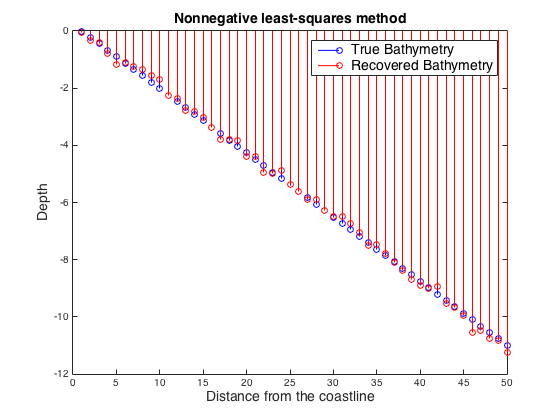
\includegraphics[scale=0.6]{img/NonLS_linear.png} 
\caption{Nonnegative least-squares method reconstruction of depth $\mathbf{h}$ using the dummy dataset.}
\label{nonLS_fig}
\end{figure}
\item[(2)]  \textit{Trust-Region-Reflective method:}  \verb|lsqnonlin(@(h) A * h - b, zeros(N,1),| \\ \verb|zeros(N,1),inf(N,1), options)|. Note that the reconstruction of $\mathbf{h}$ is restricted to the positive x-axis using the function arguments. The residual norm error of this reconstruction is $4.32 \times 10^{-10}$. 
\begin{figure}[H]
\center
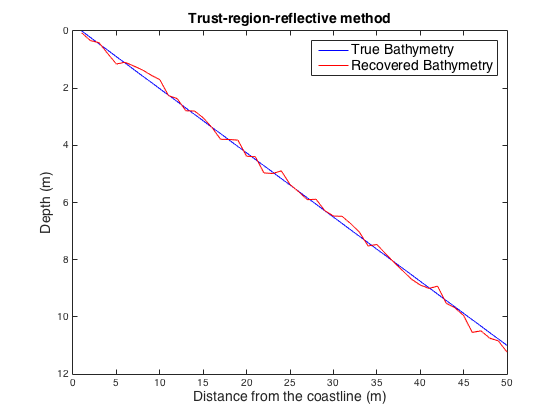
\includegraphics[scale=0.6]{img/trust_region_linear.png} 
\caption{Trust-Region-Reflective method reconstruction of depth $\mathbf{h}$ using the dummy data.}
\label{trust_region_fig}
\end{figure}
\item[(3)]  \textit{Levenberg-Marquardt (LM) method:}  
\verb|lsqnonlin(@(h) A * h - b, 'Algorithm',| \\ \verb|'levenberg-marquardt')|
Residual norm error for this reconstruction is $6.39 \times 10^{-13}$. It should be noted that the Levenberg-Marquardt algorithm does not handle bounded constraints. 
\begin{figure}[H]
\center
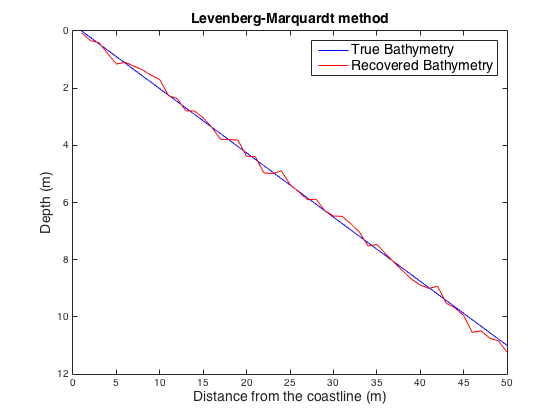
\includegraphics[scale=0.6]{img/LM_linear.png} 
\caption{Levenberg-Marquardt (LM) method reconstruction of depth $\mathbf{h}$ using the dummy data.}
\label{LM_fig}
\end{figure}
\item[(4)]  \textit{Interior-point method:} \verb|fmincon(f, zeros(N,1), [],[],[],[], zeros(N,1), inf(N,1))|. Residual norm error for the sample dummy data set  with $\nu = 0.1$ is $1.29$. 
\begin{figure}[H]
\center
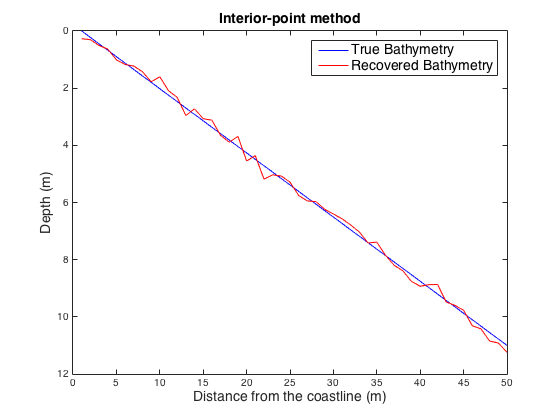
\includegraphics[scale=0.6]{img/fmincon_linear.png} 
\caption{fmincon method reconstruction of depth $\mathbf{h}$ using the dummy data.}
\label{LM_fig}
\end{figure}
\end{itemize}



\subsection{ Tikhonov Regularization}\label{TikRegMethod}

Although the ordinary least squares solution can deal with well-posed problems (i.e. the solution exist and unique), it might yield into a unstable solutions in the presence of a small noise in the measurements. Due to the ill-conditioned nature of the forward operator matrix $\mathbf{A}$, the noise components of the observations can be amplified and leads into a drastic change in the solution \cite{Tuys2014}. To overcome this problem, we use propose the use \textit{regularization}. The Tikhonov regularization is one of the most widely used regularization techniques in the inverse problems community. It couples the least squares term in \eqref{LS} with a additional regularization term as defined by 
\begin{equation}\label{eq:TR}
\mathbf{\hat{h}} = \underset{\mathbf{h} \in \mathbb{R}^n}{\arg \min} \ \ \|  \mathbf{A}\mathbf{h} -  \mathbf{d} \|_2^2  +  \alpha \| \mathbf{h}\|_2^2
\end{equation}
where $\alpha$ is the regularization parameter ($>0$), which balances the trade-off between data fidelity term (i.e, the least squares term) and the regularization term $\| \mathbf{h}\|_2^2$. %In particular, while the generalized solution strives to fit to the data, the noise components of the observations can be amplified by the forward operator. This leads into so the solution may drastically change. This behavior is due to the ill-conditioned nature of the forward operator matrix $\mathbf{A}$. 
Last but not least, the ordinary least squares method can not incorporate any prior knowledge about the bathymetry, for e.g., any known depths near the shore. However, If we have  some prior depth estimate $\mathbf{h}_p$ for the $\mathbf{h}_t$, then the Tikhonov regularized solution with the prior information can be written as
\begin{equation}\label{eq:TR-prior}
\mathbf{\hat{h}} = \underset{\mathbf{h} \in \mathbb{R}^n}{\arg \min} \  \|  \mathbf{A}\mathbf{h} -  \mathbf{d} \|_2^2  +  \alpha \| \mathbf{h} -  \mathbf{h}_p\|_2^2,
\end{equation}
where $\alpha$ is a regularization parameter $(>0)$. To test this method in \eqref{eq:TR-prior}, Tikhonov method is implemented and tested with sample data set with $\nu = 0.2$. This reconstruction of depth has 0.038 residual norm error. Note that the \verb|tikhonov| Matlab\textsuperscript{\textregistered} function requires the matrix $\mathbf{A}$ explicitly in order to solve the regularized minimization problem but the Tikhonov method can be applied through the \verb|fmincon| algorithm when $\mathbf{A}$ is not available. 

\begin{figure}[H]
\center
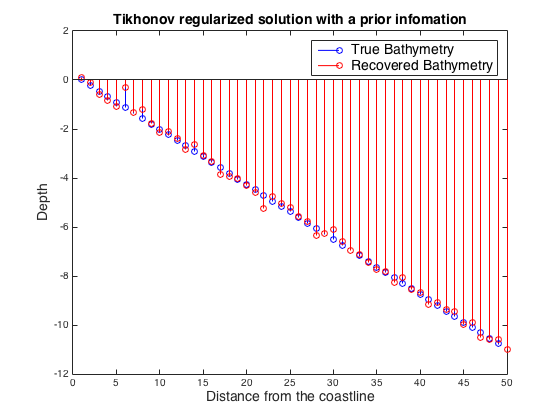
\includegraphics[scale=0.6]{img/Tikhnove_reg.png} 
\caption{The \textit{tikhonov }Matlab\textsuperscript{\textregistered} function reconstruction of the depth using the dummy data.}
\label{TR-recon}
\end{figure}

%In order to use the \verb|tikhonov| Matlab function to solve \eqref{eq:TR} or \eqref{eq:TR-prior}, the matrix $\mathbf{A}$ in should be explicitly known as a matrix. However, according to the our model derivation, forward model is nonlinear and it can not be wrtting  Therefore, we have to use some general Matlab 

%Reference: I found a MATLAB package for analysis and solution of discrete ill-posed problems, which is available in http://www2.imm.dtu.dk/~pcha/Regutools/\\








%\subsection{Help}
%
%LSQR method: $\hat{\Psi}$ = lsqr(A,d,tol,maxit) it attempts to solve the least squares solution x that minimizes norm$(\mathbf{d}-\mathbf{A\Psi})$ Note that $\mathbf{A}$ need not be square.
%
%
%Conjugate gradients: $\hat{\Psi}$ = cgs(A,b) attempts to solve the system of linear equations $\mathbf{A}\mathbf{\Psi} -  \mathbf{d}$ for $\Psi$.
%
%
%why fmincon: \url{http://www.mathworks.com/help/optim/ug/choosing-a-solver.html#bsbwxm7}

